% TODO: make mfourl bold here but not in TOC.
% TODO: check out sec-075-newEBE.tex
% \subsection{Per-Event Relative Mass Error Categorization}
\subsection{Improving Event-by-Event \mfourl Uncertainty}
\label{sec:ebe}
TODO:REWORD
For each event, the uncertainty on the \mfourl value (\mfourlerr) is used directly in the \Zone constraint (Sec.~\ref{}).
By improving the precision on the \mfourlerr 
Per-event four-lepton uncertainties are used for (a) performing the \Zone constraint and (b) in the measurement of \mH so that better-measured events are given higher weights in the likelihood fit.
Individual lepton uncertainty on momentum measurement can be predicted on a per-lepton 
basis. In the case of muons, the full error matrix is obtained using muon track fit; for the electrons,
instead, the momentum error is estimated from the combination of the ECAL and tracker measurement, 
neglecting the uncertainty on the track direction from the GSF fit. \\
The uncertainty on the kinematics at the per-lepton level is then propagated to the four-lepton case 
to predict the mass error on an event-by-event basis, using the following approach.\\
Each $\delta m_{i}$, corresponding to individual lepton momentum variation, is calculated separately 
and then the measured resolution on the invariant mass of the four leptons is taken as the quadrature sum 
of the four individual $\delta m_{i}$:
\[
m_{0} = F(p_{T1}, \phi_{1},\eta_{1}; p_{T2}, \phi_{2},\eta_{2}; p_{T3}, \phi_{3}, \eta_{3}; p_{T4}, \phi_{4},\eta_{4})
\]
\[\delta m_{i} = F(...; p_{Ti} + \delta p_{Ti}, \phi_{i}, \eta_{i}; ...) - m_{0} \quad
\]
\[
\delta m = \sqrt{\delta m_{1}^2 + \delta m_{2}^2 + \delta m_{3}^2 + \delta m_{4}^2}
\]

%=== Can't get the below to be centered...
% \begin{align*}
%         m_0 = F(
%         p_{T1}, \phi_1, \eta_1;
%         p_{T2}, \phi_2, \eta_2;
%         p_{T3}, \phi_3, \eta_3;
%         p_{T4}, \phi_4, \eta_4
%         )
%         \\
%         \delta m_i = F(...; p_{Ti} + \delta p_{Ti}, \phi_i, \eta_i; ...) - m_0
%         \\
%         \delta m = \sqrt{
%         (\delta m_1)^2 + (\delta m_2)^2 + (\delta m_3)^2 + (\delta m_4)^2
%         }
% \end{align*}
% TODO: Check with Filippo if these are MC or data.
The full error matrices ($\delta p_{T}/p_{T}$, $\eta$) for muons and electrons, separately, are shown in Fig.~\ref{fig:2D_Mpas_vs_eta} for all years.
\begin{multiFigure}
    \centering

    \addFigure{0.32}{figures/higgsmassmeas/ebe/2016_vs_eta_muon.pdf}
    \addFigure{0.32}{figures/higgsmassmeas/ebe/2016_vs_eta_ele_ECAL.pdf}
    \addFigure{0.32}{figures/higgsmassmeas/ebe/2016_vs_eta_ele_tracker.pdf}

    \addFigure{0.32}{figures/higgsmassmeas/ebe/2017_vs_eta_muon.pdf}
    \addFigure{0.32}{figures/higgsmassmeas/ebe/2017_vs_eta_ele_ECAL.pdf}
    \addFigure{0.32}{figures/higgsmassmeas/ebe/2017_vs_eta_ele_tracker.pdf}

    \addFigure{0.32}{figures/higgsmassmeas/ebe/2018_vs_eta_muon.pdf}
    \addFigure{0.32}{figures/higgsmassmeas/ebe/2018_vs_eta_ele_ECAL.pdf}
    \addFigure{0.32}{figures/higgsmassmeas/ebe/2018_vs_eta_ele_tracker.pdf}
    \captionof{figure}
        [Scatterplot of the relative lepton \pt error vs $\eta$ for muons and electrons]
        {Scatterplot of the relative lepton \pt error vs $\eta$ for muons (left column), ECAL driven electrons (middle column), and tracker driven electrons (right column) for 2016 (top row), 2017 (middle row), and 2018 (bottom row) data.}
    \label{fig:2D_Mpas_vs_eta}
\end{multiFigure}
% \begin{figure}[!htbp]
% 	\begin{center}
% %		\subfloat[][2016]
% %		   {		
%                     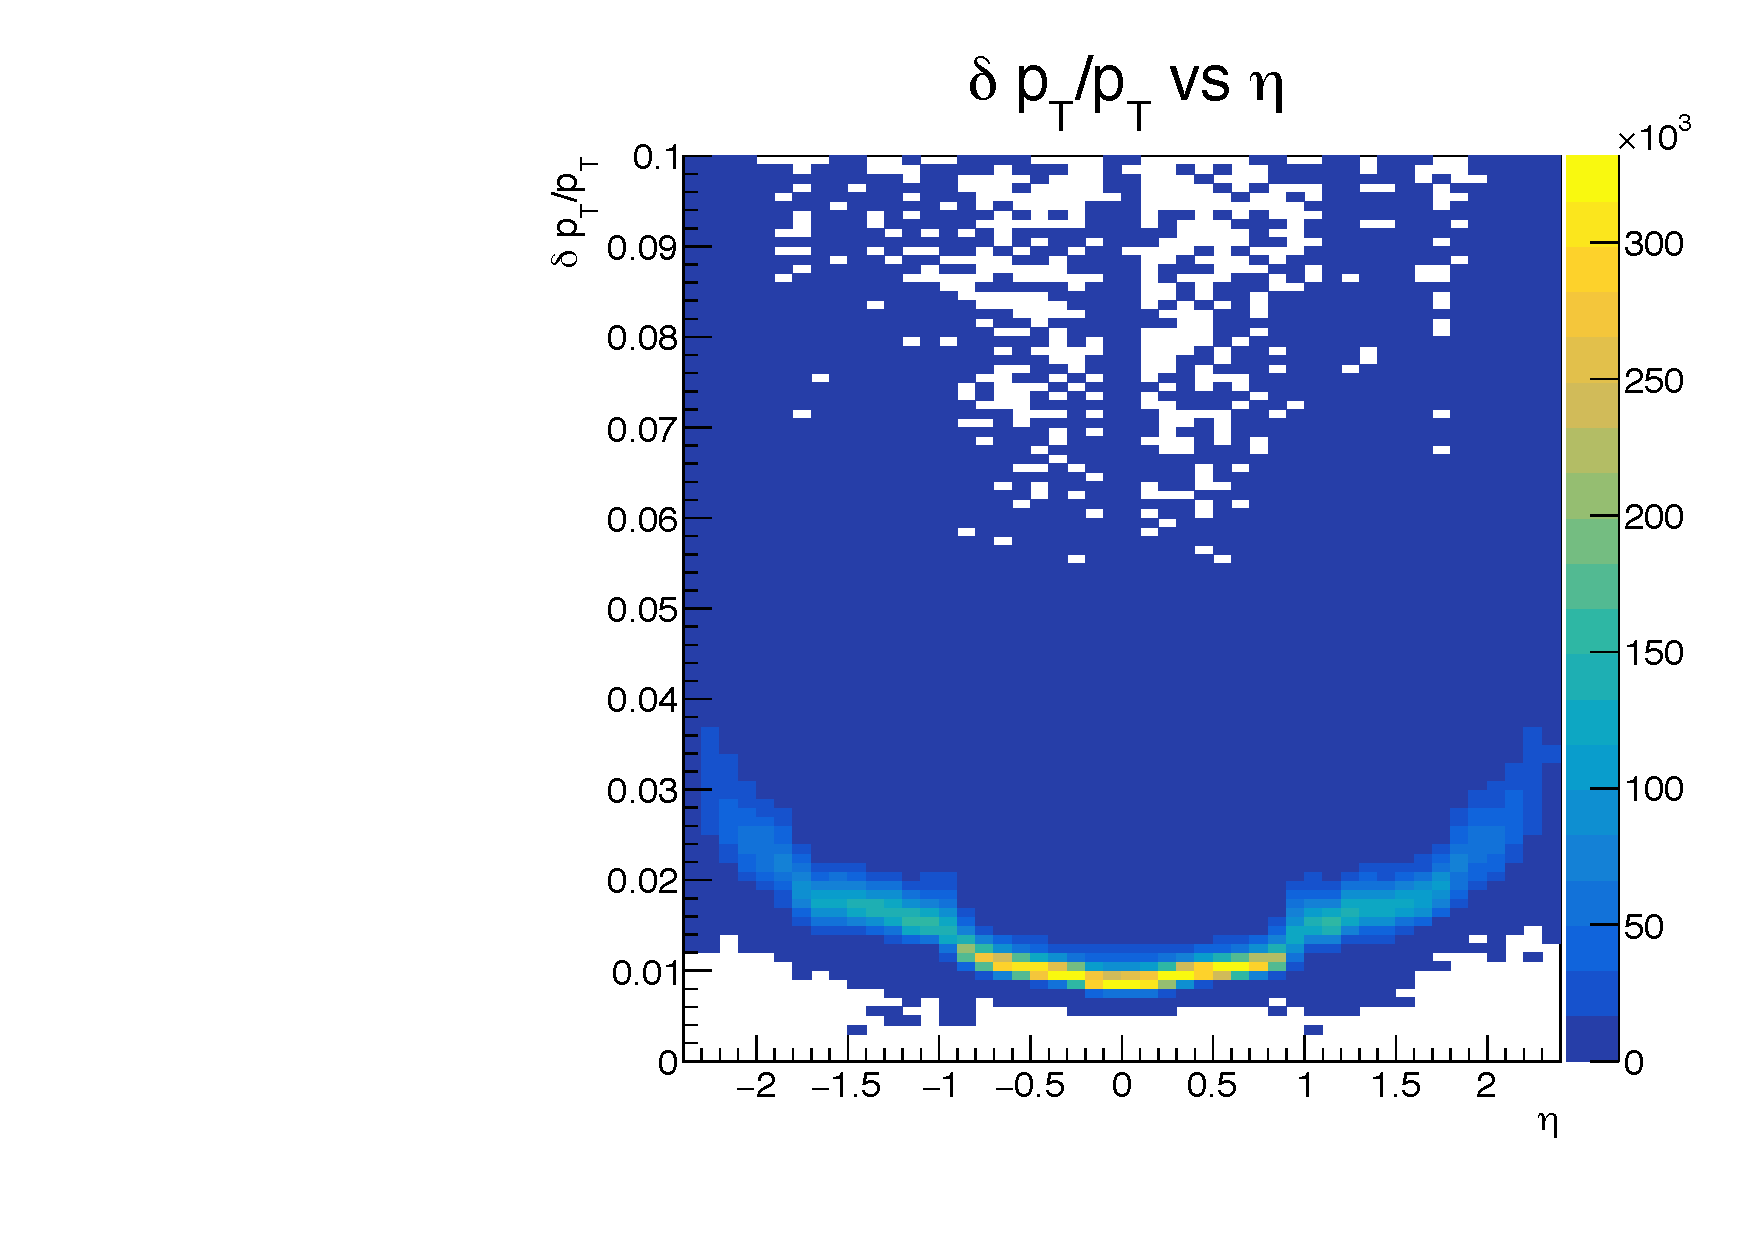
\includegraphics[width=0.32\textwidth]{Figures/EBE/2016_vs_eta_muon.pdf}
% 					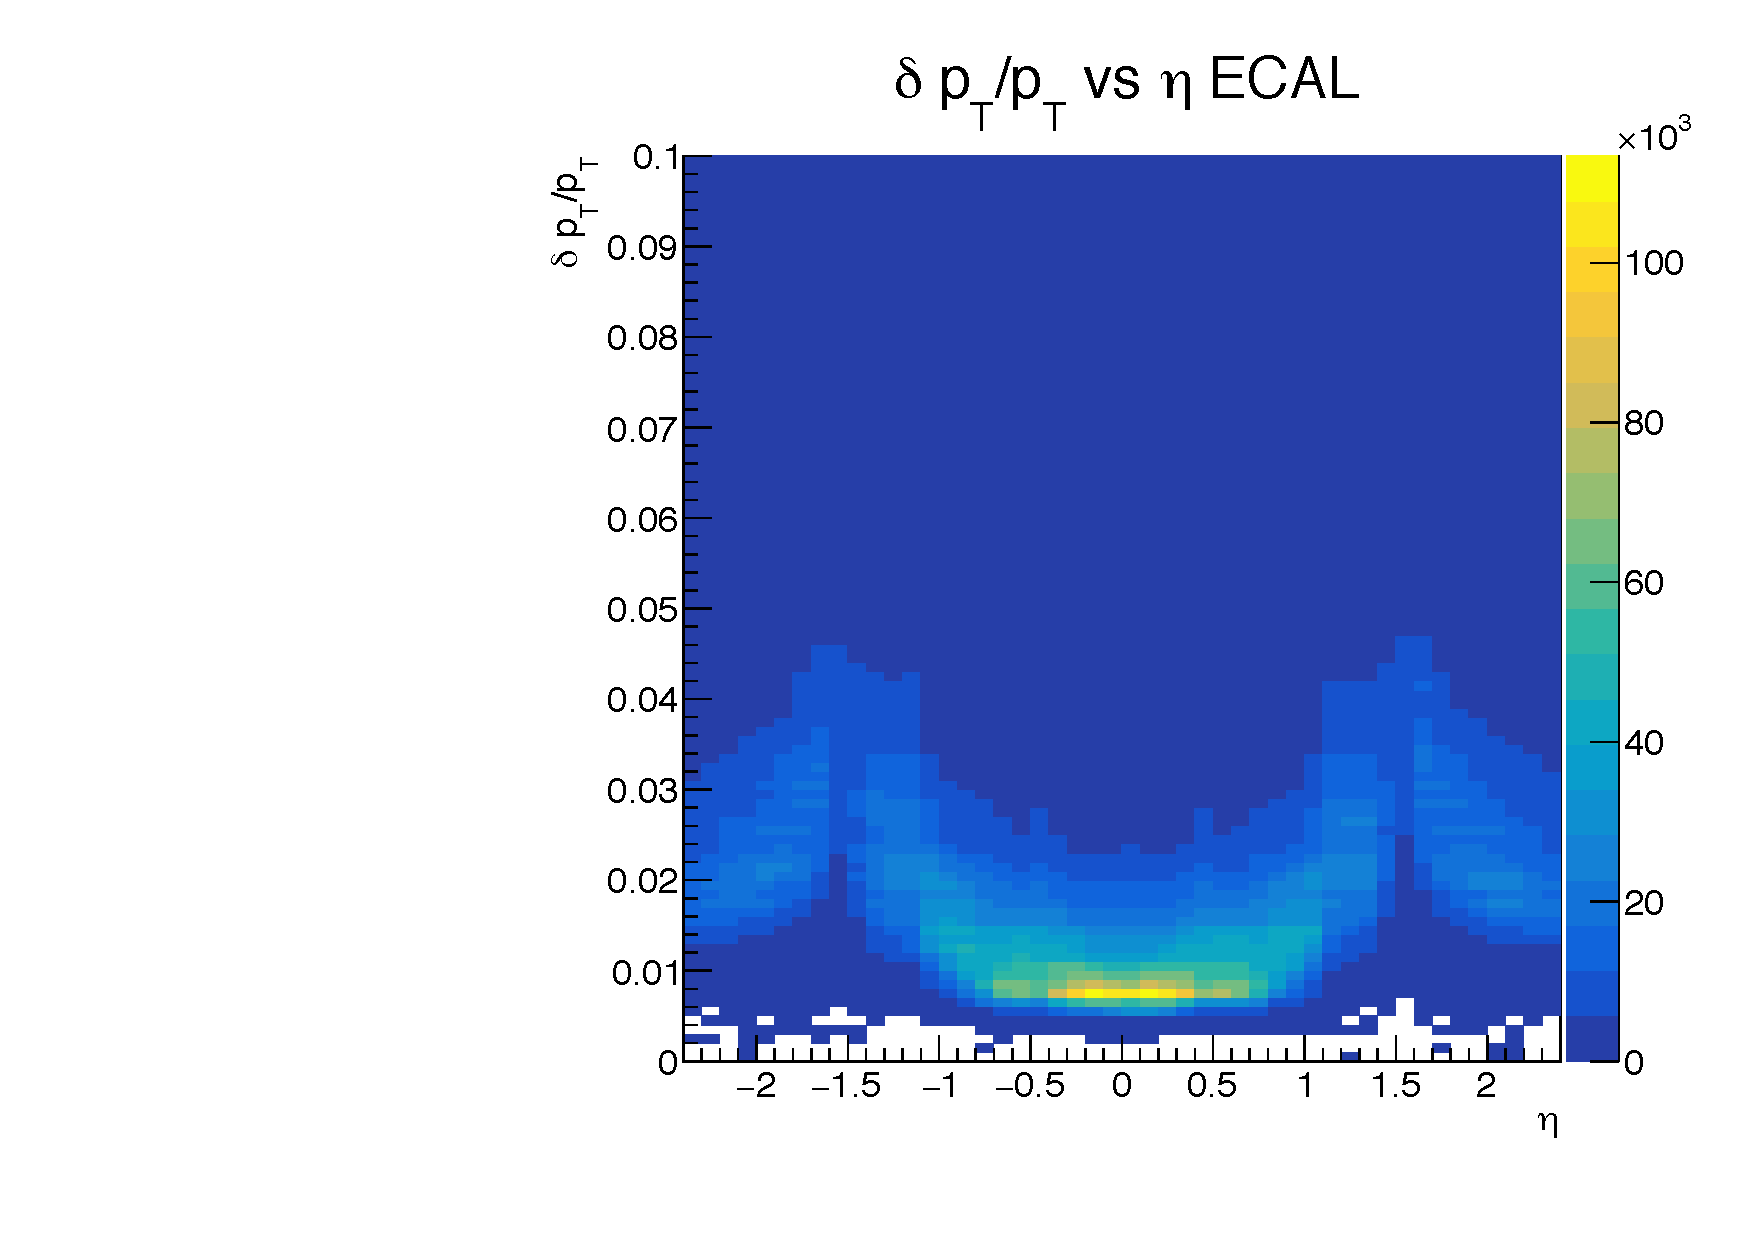
\includegraphics[width=0.32\textwidth]{Figures/EBE/2016_vs_eta_ele_ECAL.pdf} 
% 					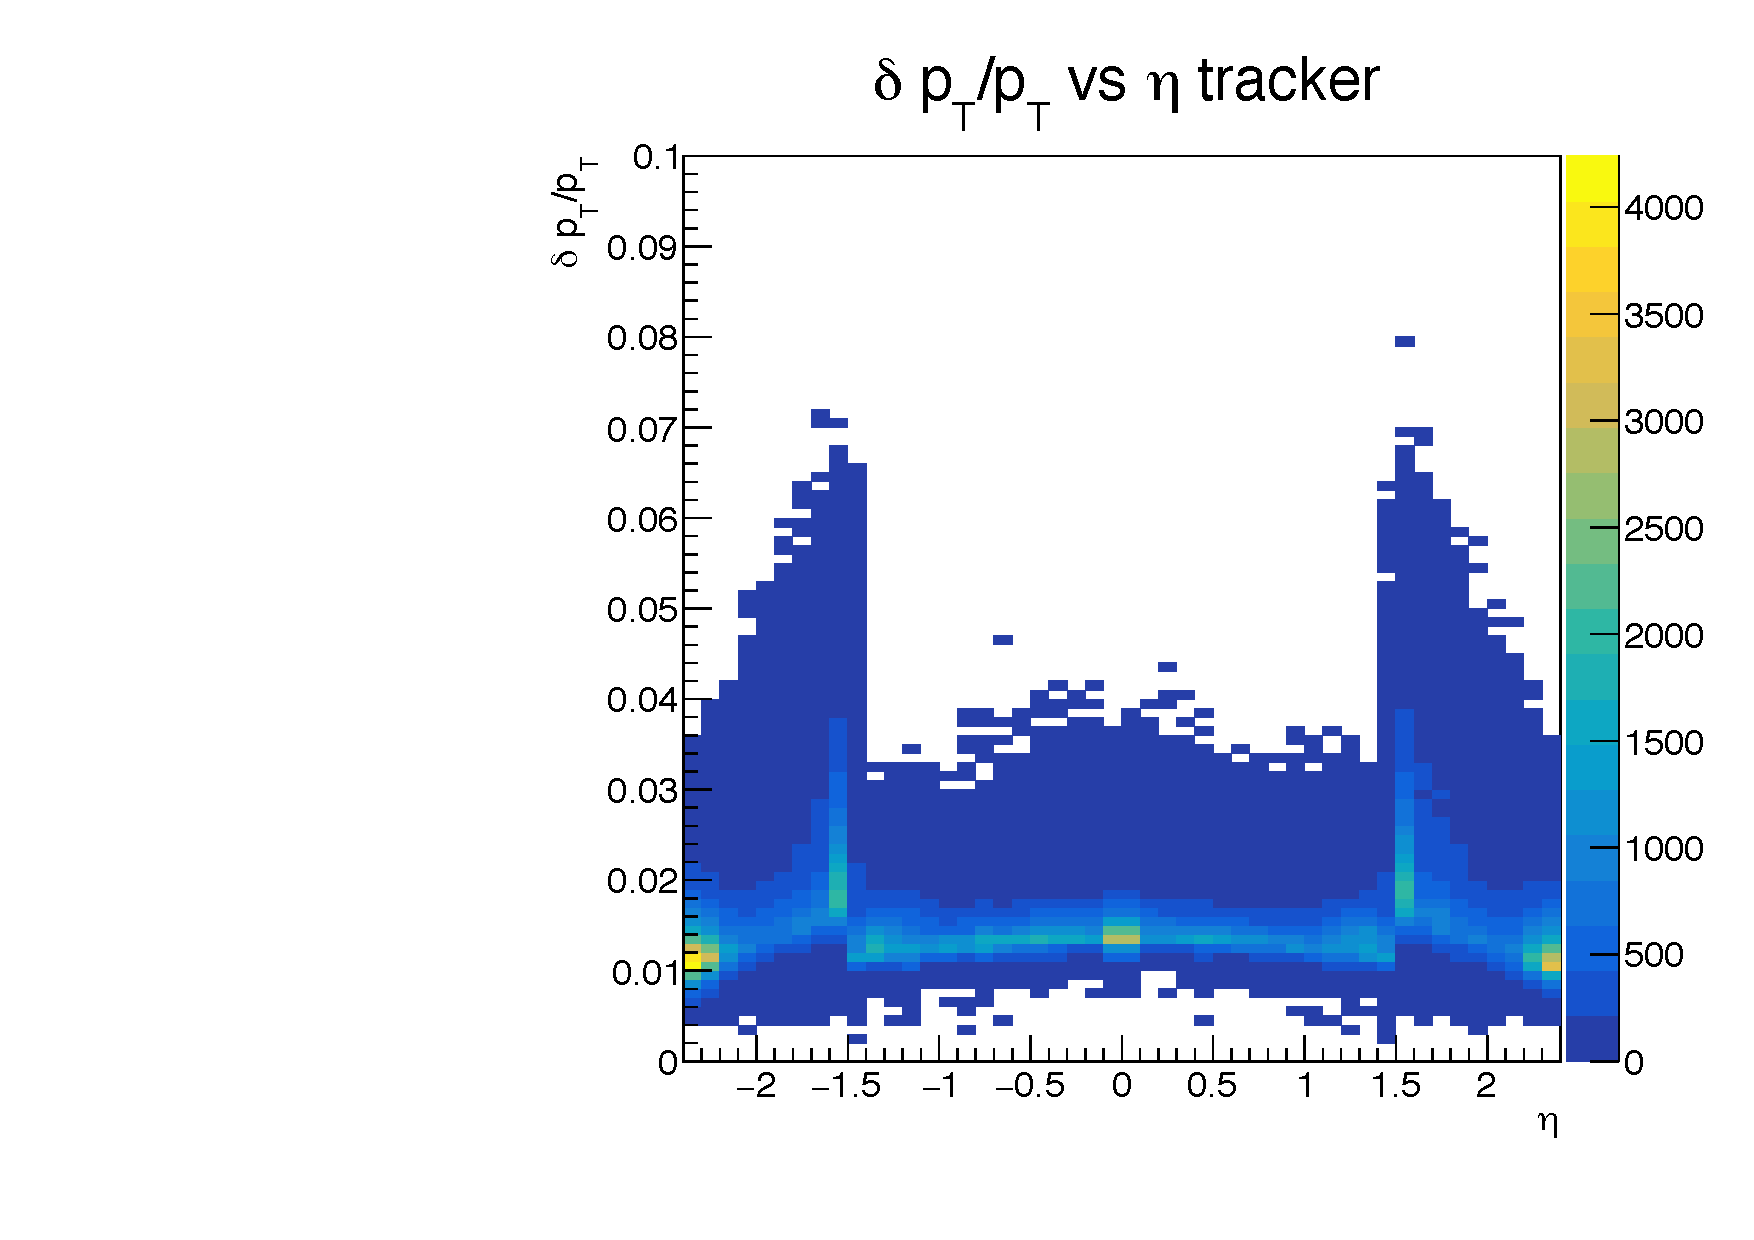
\includegraphics[width=0.32\textwidth]{Figures/EBE/2016_vs_eta_ele_tracker.pdf}
% %			}\\
% %		\subfloat[][2017]
%             % {
% 		    		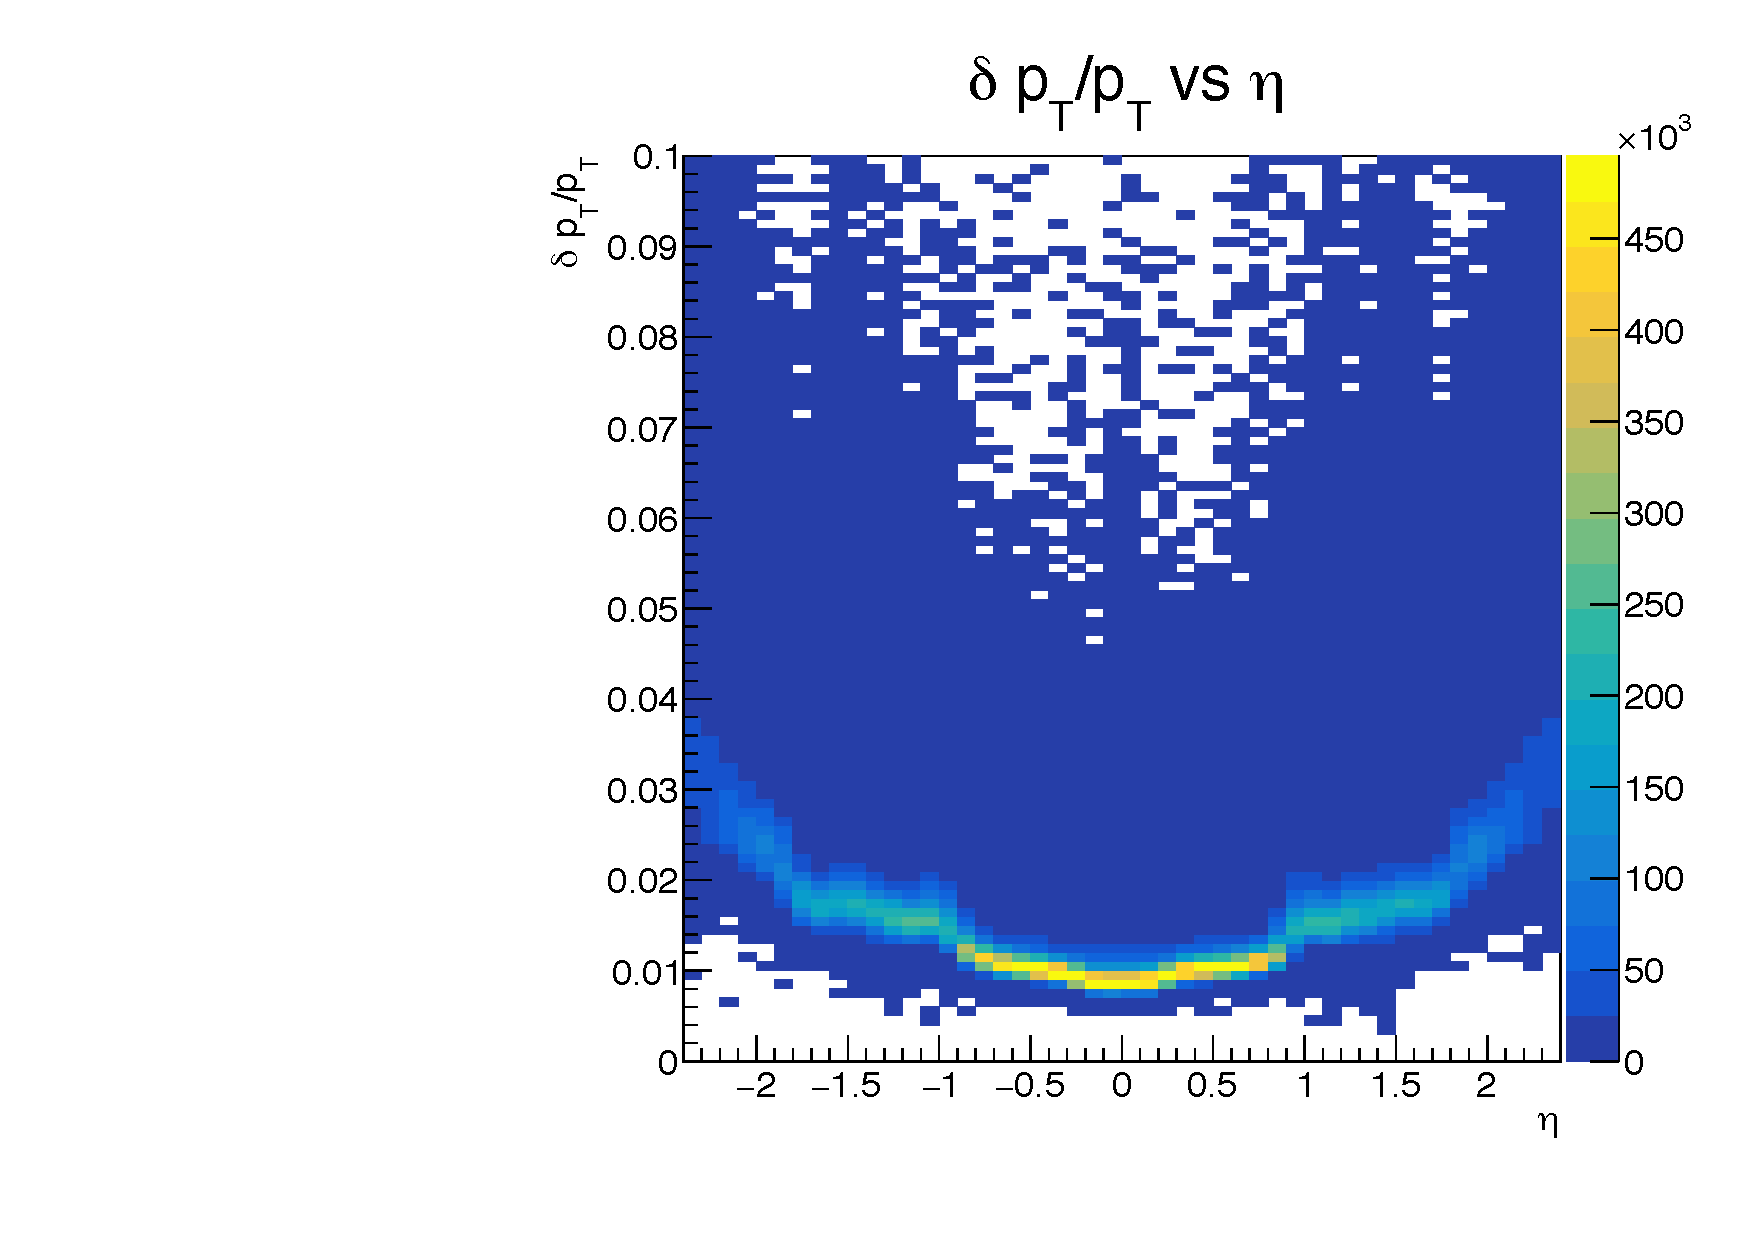
\includegraphics[width=0.32\textwidth]{Figures/EBE/2017_vs_eta_muon.pdf}
% 					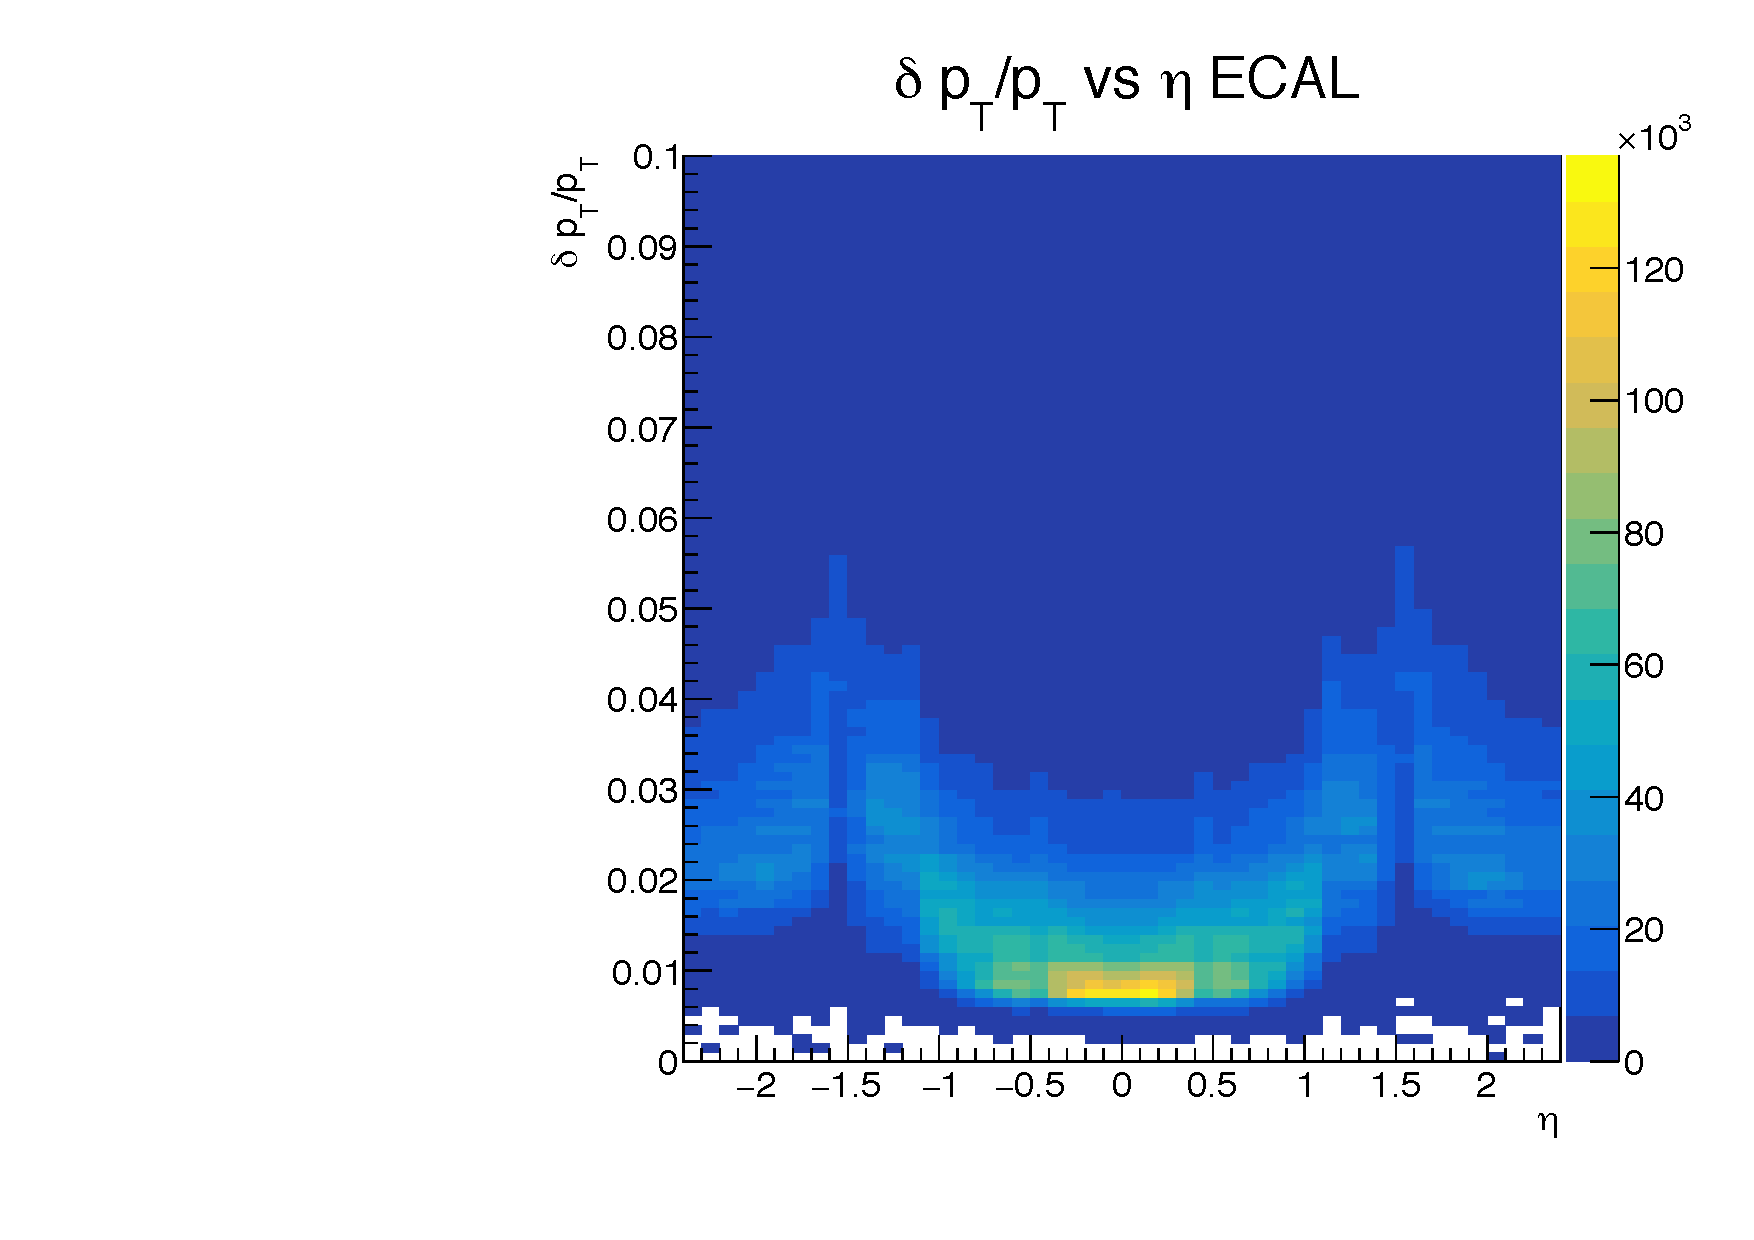
\includegraphics[width=0.32\textwidth]{Figures/EBE/2017_vs_eta_ele_ECAL.pdf} 
% 					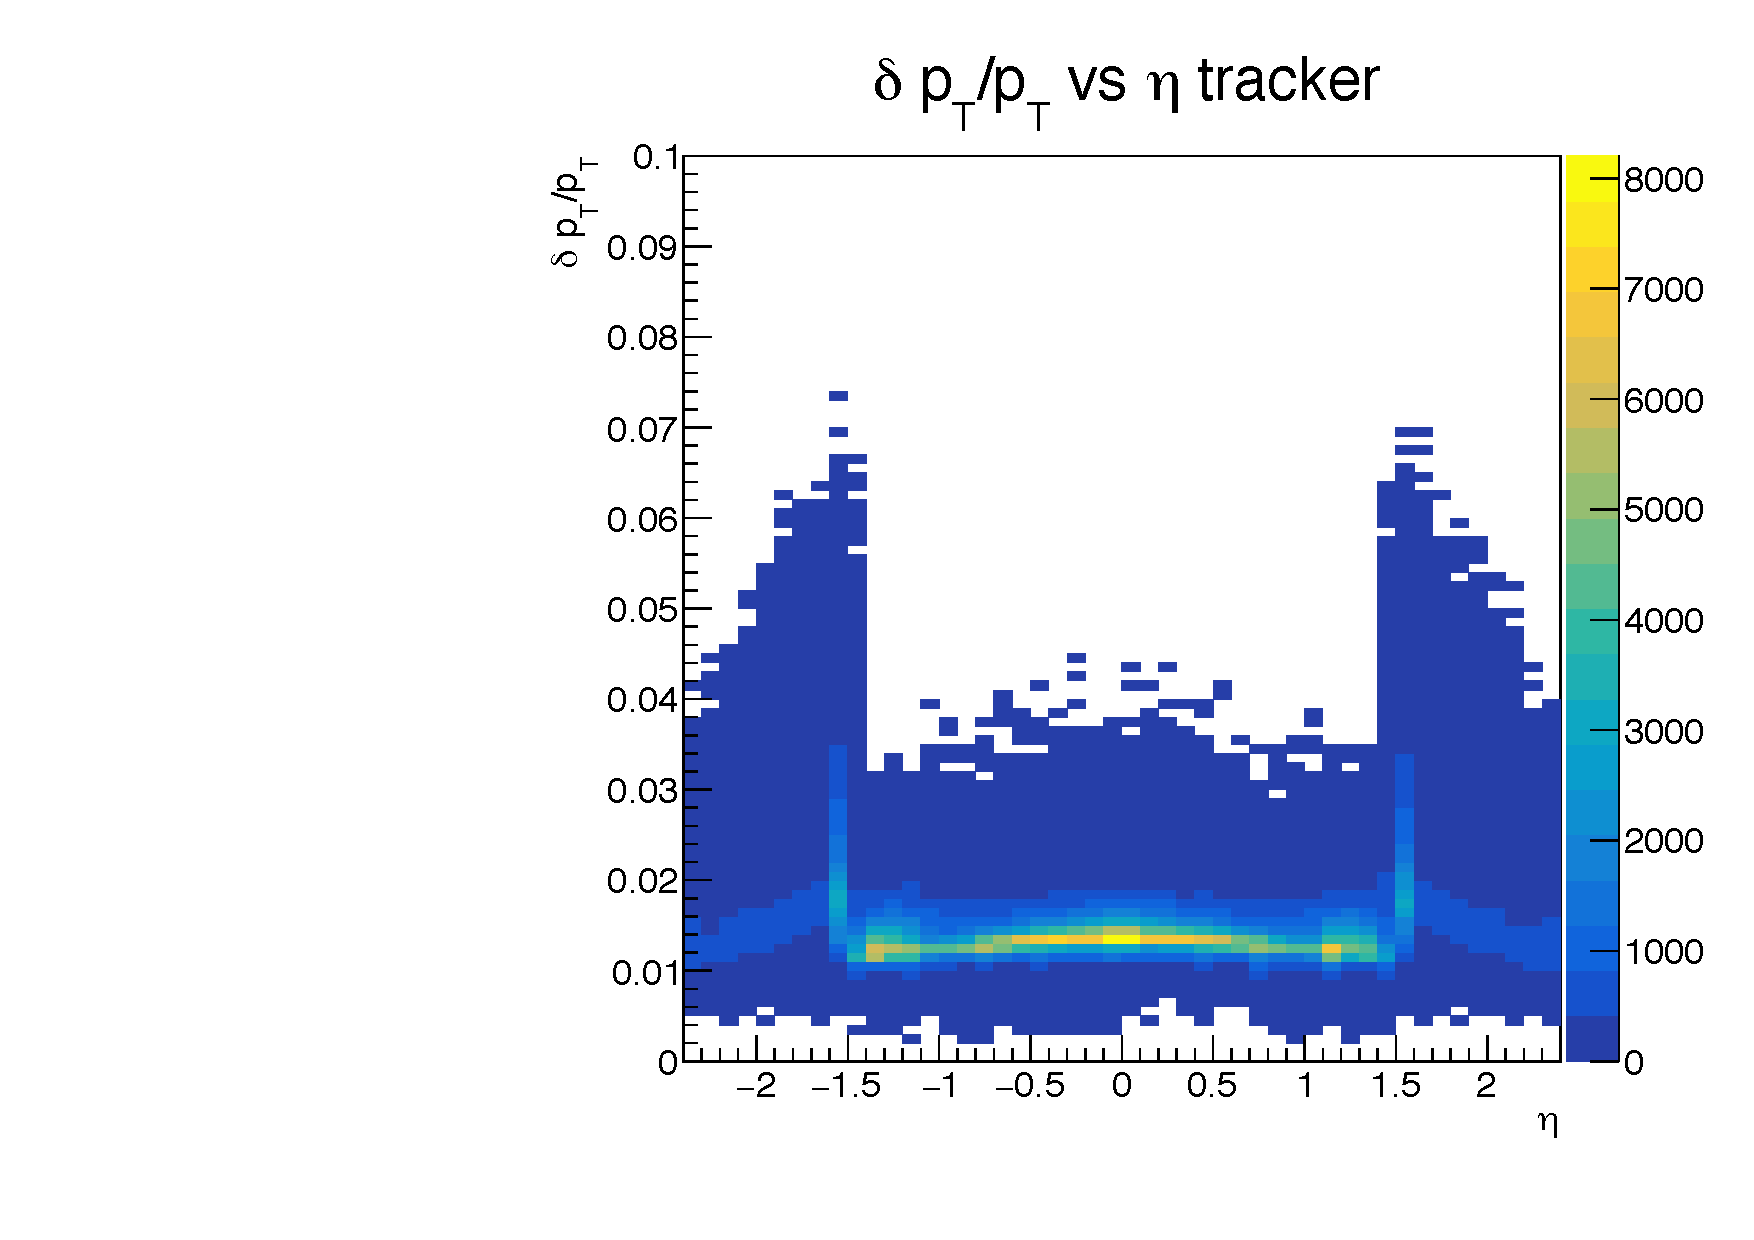
\includegraphics[width=0.32\textwidth]{Figures/EBE/2017_vs_eta_ele_tracker.pdf}
% %			}\\
% %		\subfloat[][2018]
%             % {
% 		    		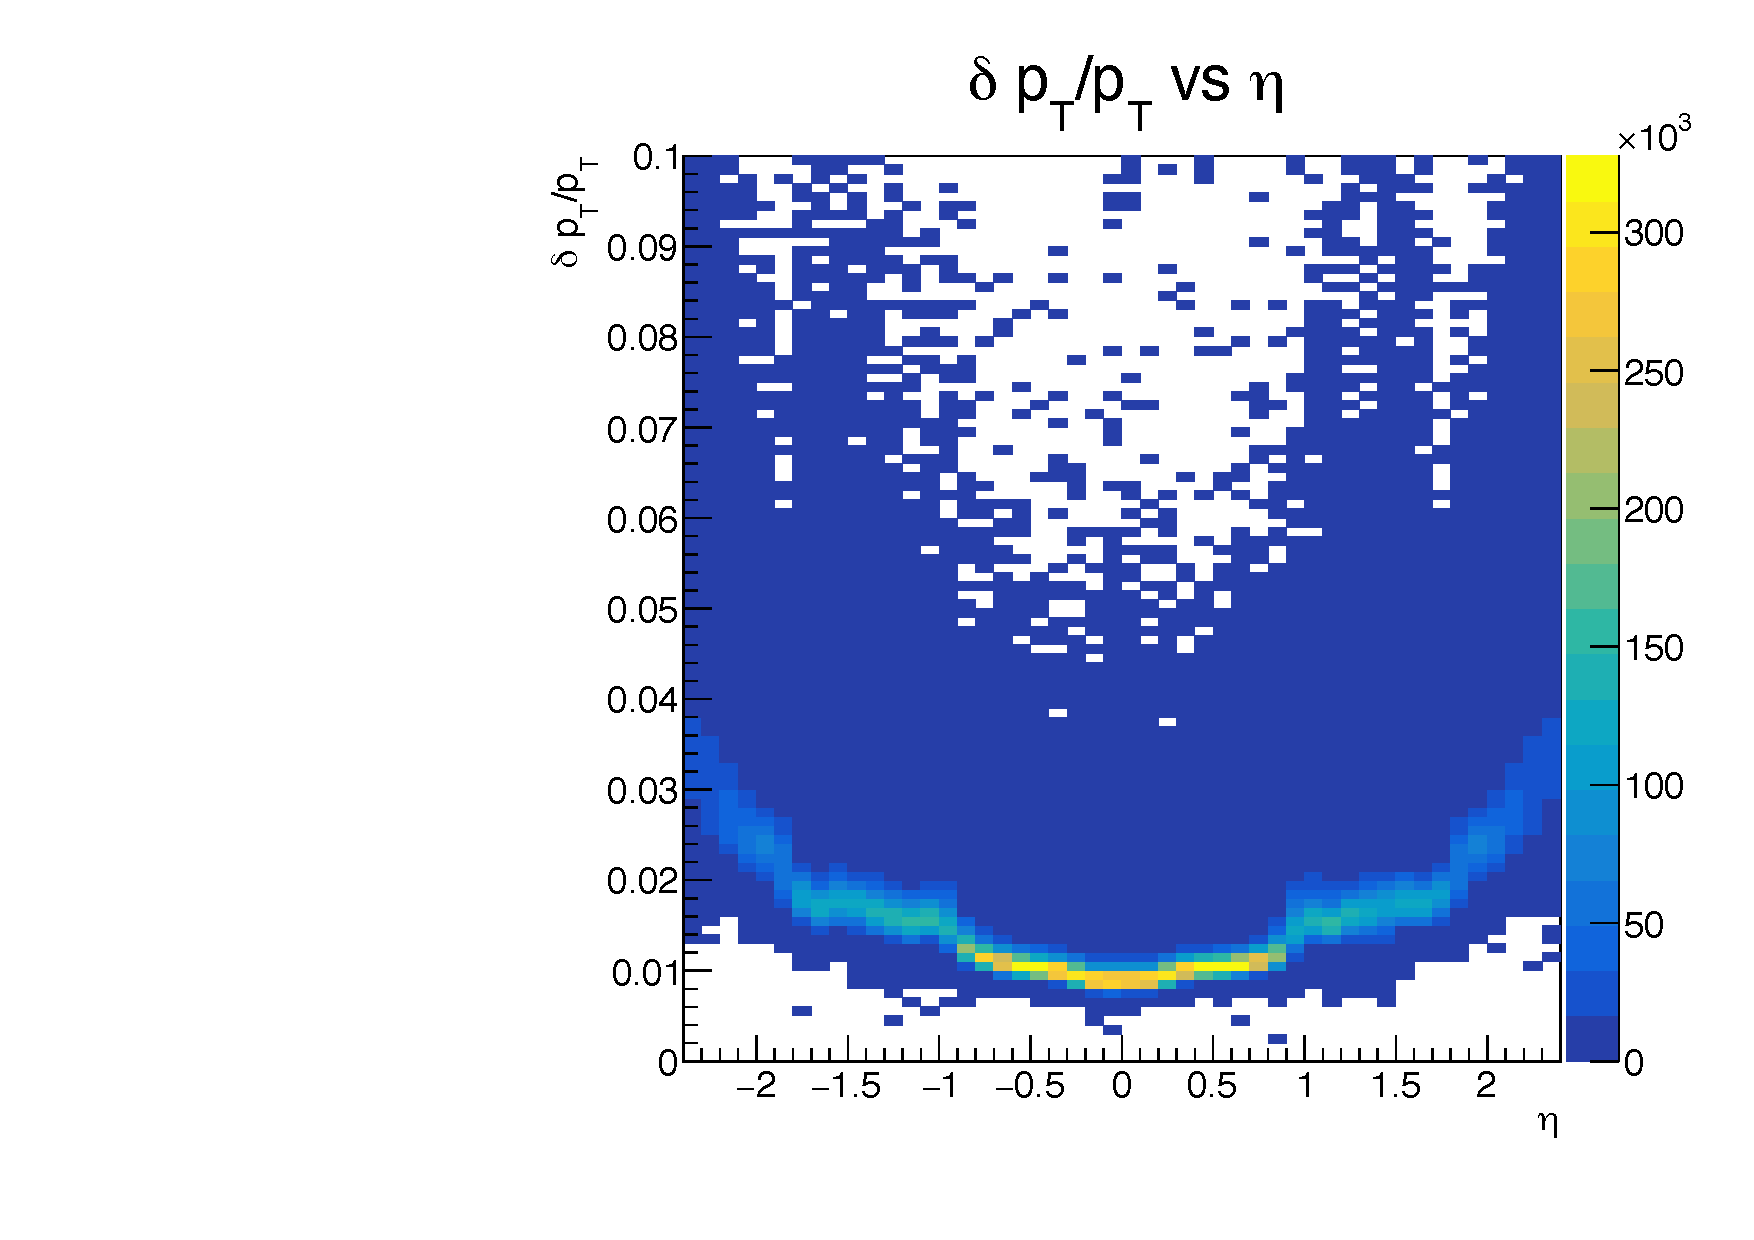
\includegraphics[width=0.32\textwidth]{figures/higgsmassmeas/ebe/2018_vs_eta_muon.pdf}
% 					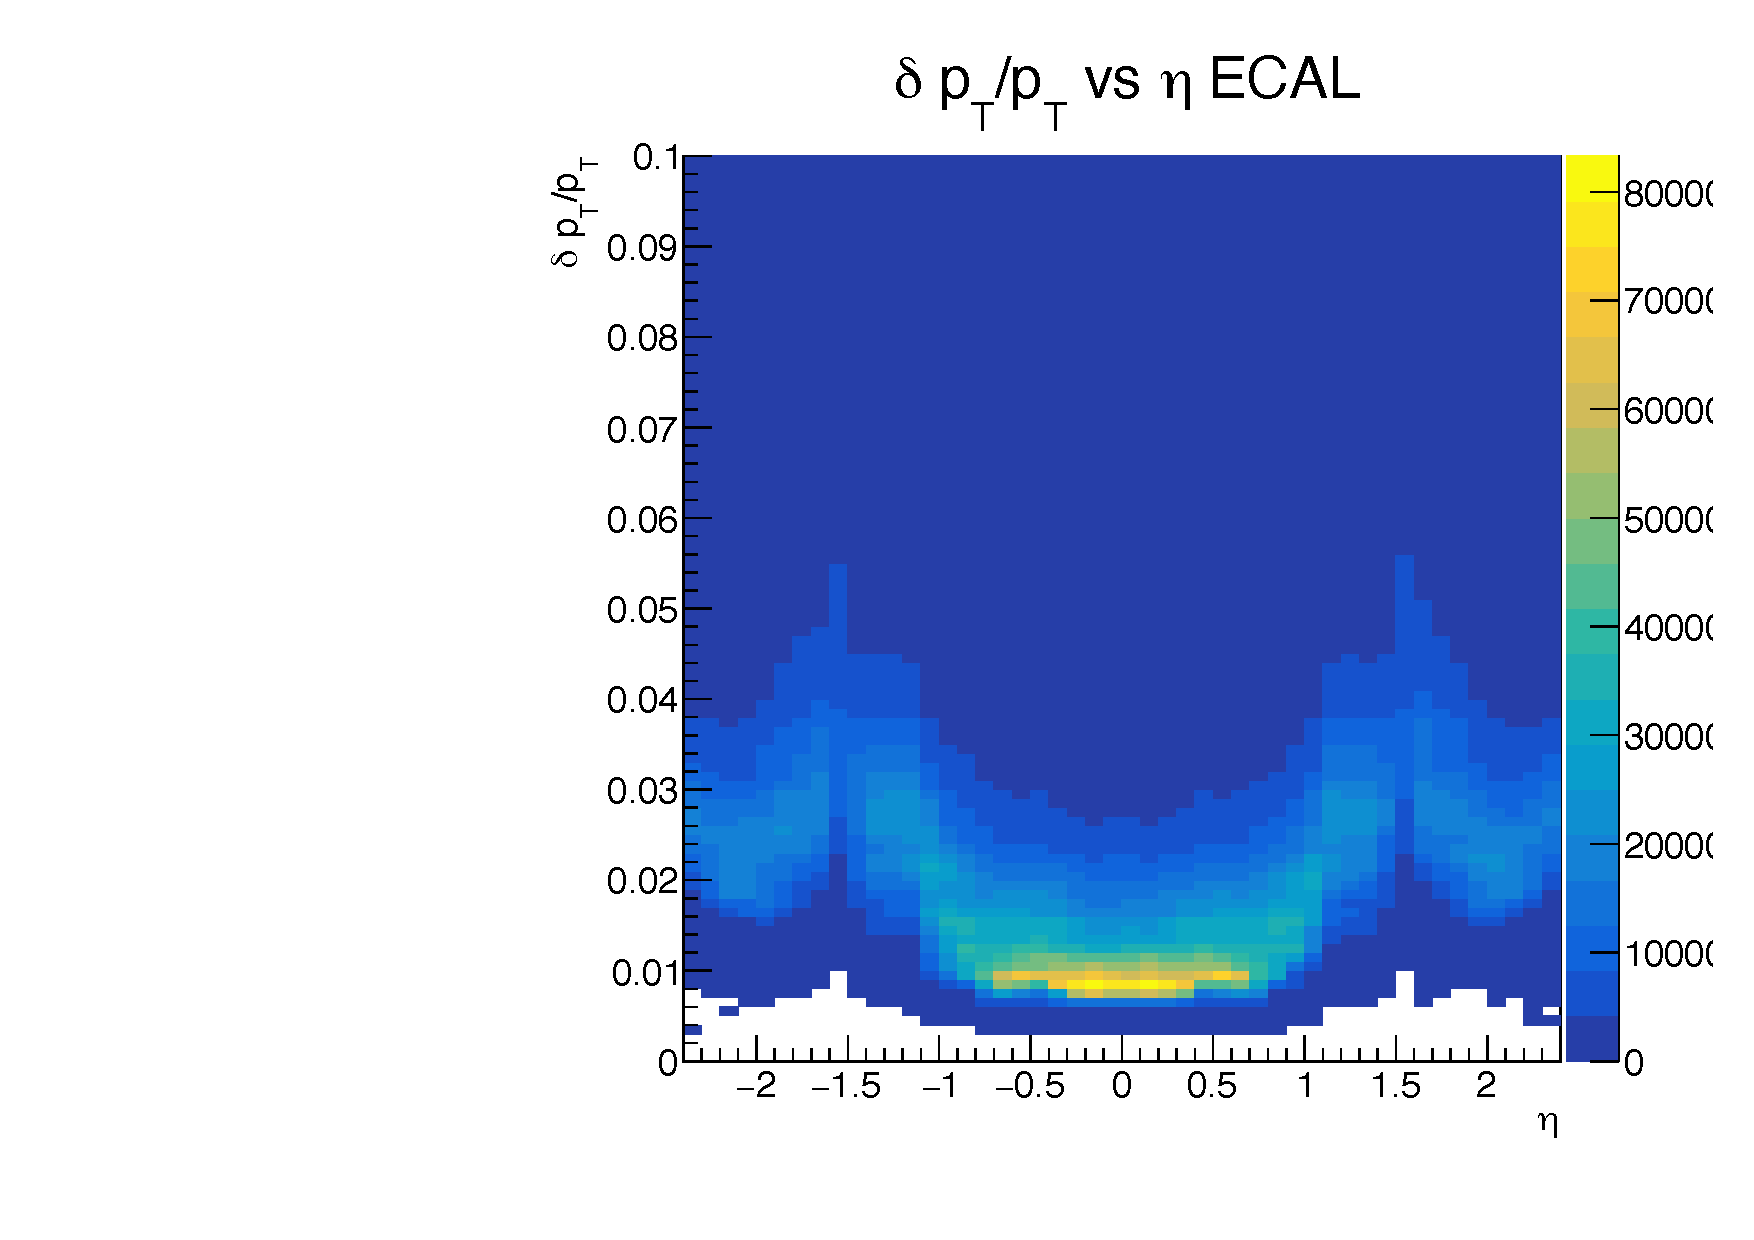
\includegraphics[width=0.32\textwidth]{figures/higgsmassmeas/ebe/2018_vs_eta_ele_ECAL.pdf} 
% 					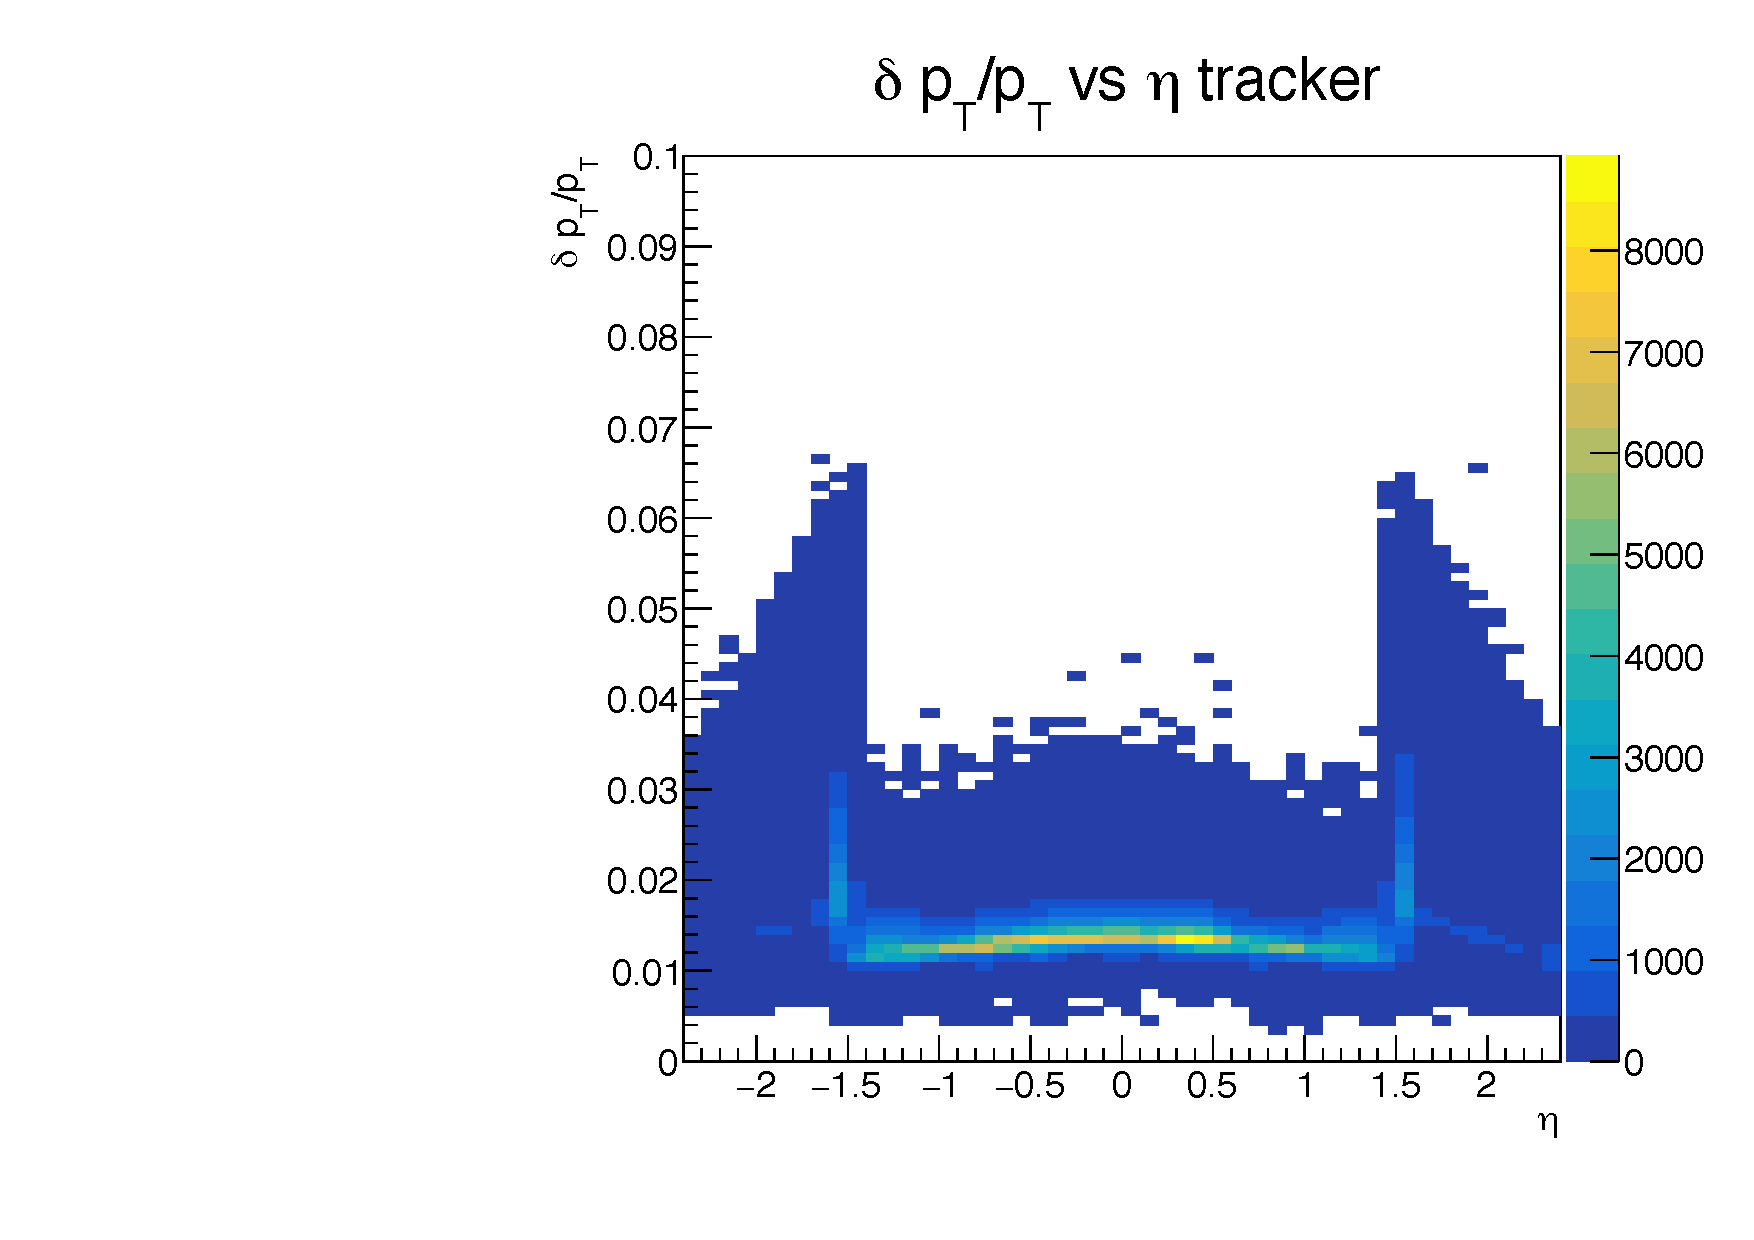
\includegraphics[width=0.32\textwidth]{figures/higgsmassmeas/ebe/2018_vs_eta_ele_tracker.pdf}
% %			}\\
% 		\caption{Scatterplot of the relative lepton \PT error vs $\eta$ for muons (left), 
% 				ECAL driven electrons (middle), and tracker driven electrons (right) for 2018 data.}
% 	\label{fig:2D_Mpas_vs_eta}
% 	\end{center}
% \end{figure}

Starting from these distributions, corrections to lepton momentum uncertainty in mutual $|\eta|$ bins are derived for muons (Fig.~\ref{fig:2D_Mpas_vs_pt_muon}), ECAL-driven electrons (Fig.~\ref{fig:2D_Mpas_vs_pt_electron_ECAL}), and tracker electrons (Fig.~\ref{fig:2D_Mpas_vs_pt_electron_tracker}) using bins of $\delta p_{T}$/$p_{T}$ \vs \abseta.
Scatterplots of $\delta p_{T}$/$p_{T}$ \vs \PT are shown in Figs.~\ref{fig:2D_Mpas_vs_pt_electron_ECAL} and~\ref{fig:2D_Mpas_vs_pt_electron_tracker}.
% Muons.
\begin{multiFigure}
    \centering
    \addFigure{0.32}{figures/higgsmassmeas/ebe/2016_vs_pt_muon_1.pdf}
    \addFigure{0.32}{figures/higgsmassmeas/ebe/2016_vs_pt_muon_2.pdf}
    \addFigure{0.32}{figures/higgsmassmeas/ebe/2016_vs_pt_muon_3.pdf}

    \addFigure{0.32}{figures/higgsmassmeas/ebe/2017_vs_pt_muon_1.pdf}
    \addFigure{0.32}{figures/higgsmassmeas/ebe/2017_vs_pt_muon_2.pdf}
    \addFigure{0.32}{figures/higgsmassmeas/ebe/2017_vs_pt_muon_3.pdf}

    \addFigure{0.32}{figures/higgsmassmeas/ebe/2018_vs_pt_muon_1.pdf}
    \addFigure{0.32}{figures/higgsmassmeas/ebe/2018_vs_pt_muon_2.pdf}
    \addFigure{0.32}{figures/higgsmassmeas/ebe/2018_vs_pt_muon_3.pdf}
    \captionof{figure}
        [words.]
        {Scatterplot of the relative lepton \PT error vs \PT for muons with $0 < \abseta < 0.9$ (left column), $0.9 < \abseta < 1.8$ (middle column), and $1.8 < \abseta < 2.4$ (right column) for 2016 (top row), 2017 (middle row), and 2018 (bottom row) data.}
    \label{fig:2D_Mpas_vs_pt_muon}
\end{multiFigure}
% ECAL electrons.
\begin{multiFigure}
    \centering
    \addFigure{0.32}{figures/higgsmassmeas/ebe/2016_vs_pt_ECAL_1.pdf}
    \addFigure{0.32}{figures/higgsmassmeas/ebe/2016_vs_pt_ECAL_2.pdf}
    \addFigure{0.32}{figures/higgsmassmeas/ebe/2016_vs_pt_ECAL_3.pdf}

    \addFigure{0.32}{figures/higgsmassmeas/ebe/2017_vs_pt_ECAL_1.pdf}
    \addFigure{0.32}{figures/higgsmassmeas/ebe/2017_vs_pt_ECAL_2.pdf}
    \addFigure{0.32}{figures/higgsmassmeas/ebe/2017_vs_pt_ECAL_3.pdf}

    \addFigure{0.32}{figures/higgsmassmeas/ebe/2018_vs_pt_ECAL_1.pdf}
    \addFigure{0.32}{figures/higgsmassmeas/ebe/2018_vs_pt_ECAL_2.pdf}
    \addFigure{0.32}{figures/higgsmassmeas/ebe/2018_vs_pt_ECAL_3.pdf}
    \captionof{figure}
        [words.]
        % TODO: Is it OK to skip over 1.0--2.0?
        {Scatterplot of the relative lepton \PT error vs \PT for ECAL-driven electrons with $0 < \abseta < 0.8$ (left column), $0.8 < \abseta < 1.0$ (middle column), and $2.0 < \abseta < 2.5$ (right column) for 2016 (top row), 2017 (middle row), and 2018 (bottom row) data.}
    \label{fig:2D_Mpas_vs_pt_electron_ECAL}
\end{multiFigure}
% Tracker electrons.
\begin{multiFigure}
    \centering
    \addFigure{0.32}{figures/higgsmassmeas/ebe/2016_vs_pt_tracker_1.pdf}
    \addFigure{0.32}{figures/higgsmassmeas/ebe/2016_vs_pt_tracker_2.pdf}
    \addFigure{0.32}{figures/higgsmassmeas/ebe/2016_vs_pt_tracker_3.pdf}

    \addFigure{0.32}{figures/higgsmassmeas/ebe/2017_vs_pt_tracker_1.pdf}
    \addFigure{0.32}{figures/higgsmassmeas/ebe/2017_vs_pt_tracker_2.pdf}
    \addFigure{0.32}{figures/higgsmassmeas/ebe/2017_vs_pt_tracker_3.pdf}

    \addFigure{0.32}{figures/higgsmassmeas/ebe/2018_vs_pt_tracker_1.pdf}
    \addFigure{0.32}{figures/higgsmassmeas/ebe/2018_vs_pt_tracker_2.pdf}
    \addFigure{0.32}{figures/higgsmassmeas/ebe/2018_vs_pt_tracker_3.pdf}
    \captionof{figure}
        [words.]
        % TODO: Is it OK to skip over 1.44--1.6?
        {Scatterplot of the relative lepton \PT error vs \PT for tracker-driven electrons with $0 < \abseta < 0.8$ (left column), $1.0 < \abseta < 1.44$ (middle column), and $1.6 < \abseta < 2.0$ (right column) for 2016 (top row), 2017 (middle row), and 2018 (bottom row) data.}
    \label{fig:2D_Mpas_vs_pt_electron_tracker}
\end{multiFigure}

\subsubsection{Procedure to Derive Corrections to $\delta \ptl$}
TODO: REWORD
To derive the corrections ($\lambda$), the dilepton invariant mass $\left( \mll \right)$ from \ztolplm events is fitted twice with a Breit--Wigner (BW) function convolved with a Crystal Ball (CB), plus an exponential function (EXP).
In this model, the BW represents the true \mZ lineshape, the CB simulates the detector effects, and the EXP describes the falling background.
When deriving the corrections, the mean and sigma of the BW have been set to the PDG values $\left( \mZ = 91.19\GeV, \; \Gamma_{\PZ} = 2.49\GeV \right)$~\cite{particle_data_group_review_2020}.
 The fit is done in the mass range [60, 120]\GeV, using only
$e^{+}e^{-}$ or $\mu^{+}\mu^{-}$ pairs.\\
The first fit is used to fix all the parameters of the functions but the $\sigma$ of the CB which is
replaced in the second fit by $\lambda$ $\times$ $\delta_{m_{Z}}$, where $\lambda$ is the 
floated parameter of the fit. 

%If statistics is large enough for a...\textbf{DECIDE HOW TO BEHAVE IN CASE OF LACK OF STATISTCS}.

The summary of $\lambda$ correction factors for electrons and muons is shown in Table~\ref{table:Lambdas}.
\begin{multiFigure}
    \centering
    \captionof{table}
    [TODO: Lambda values.]
    {TODO: Convert to proper table. ELIMINATE DATA FROM TABLE. Lambda values.}
    \addFigure{0.96}{figures/higgsmassmeas/ebe/table_lambdas.png}
    % 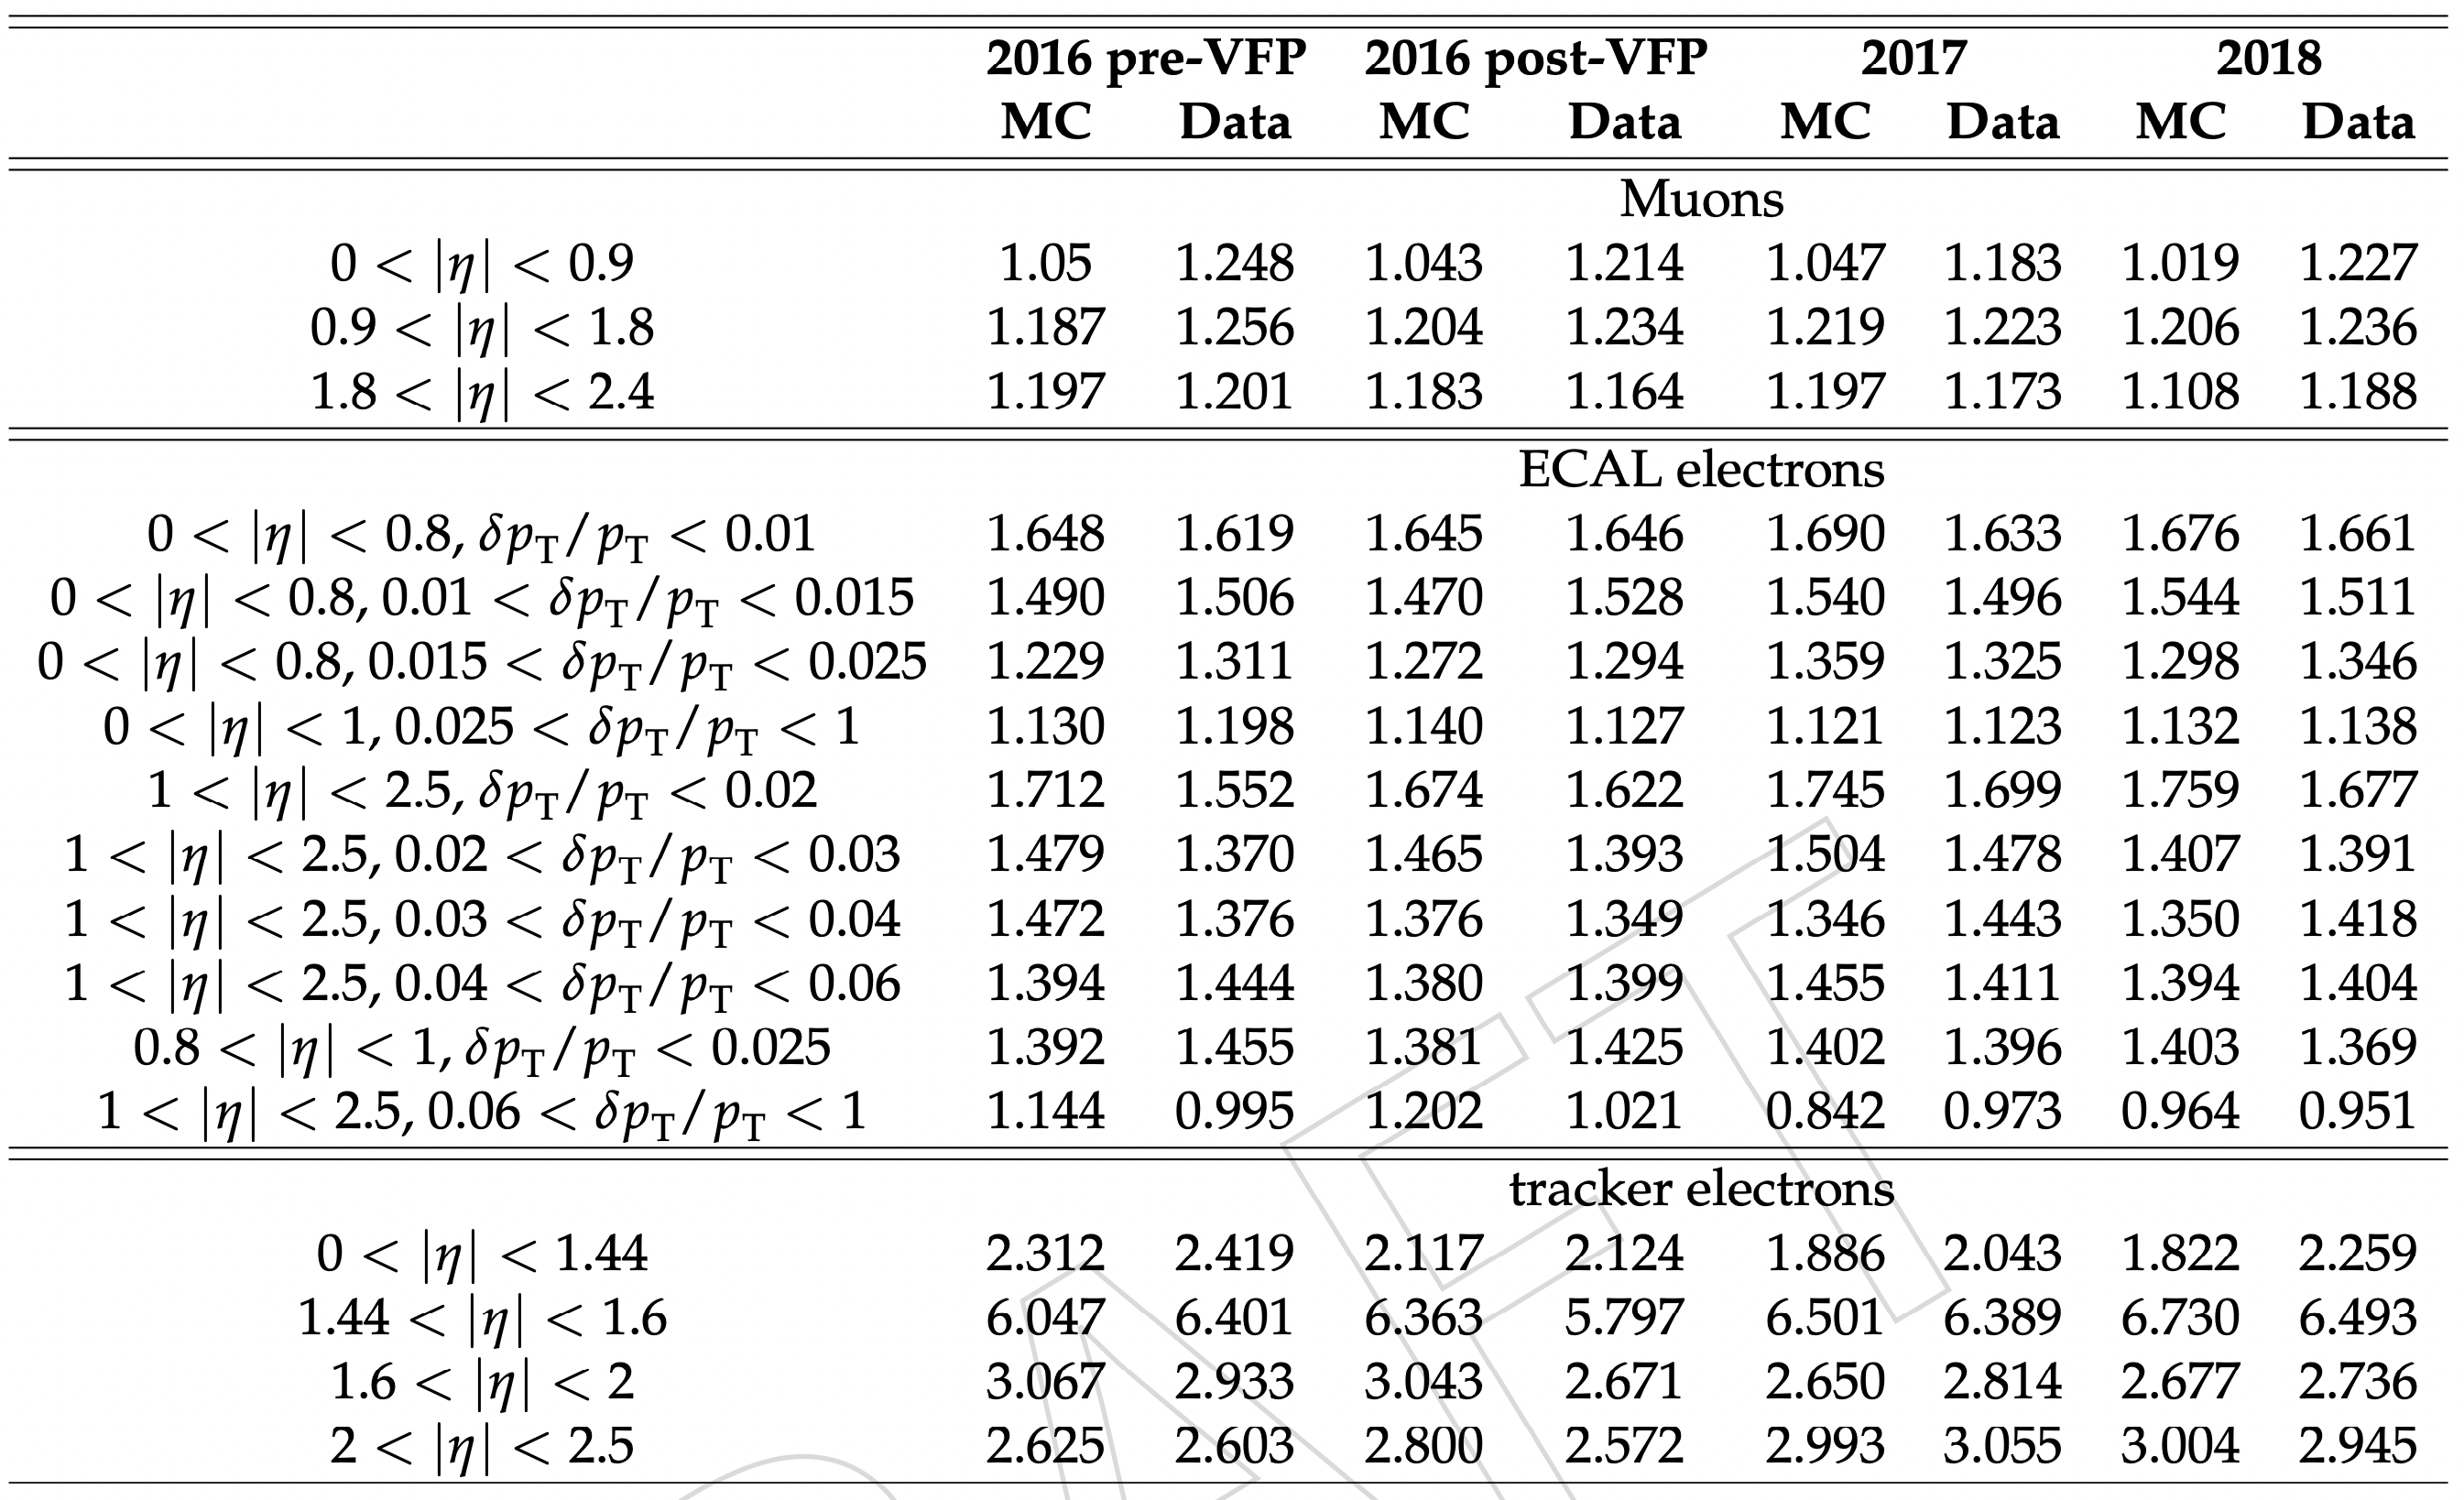
\includegraphics[width=0.96\textwidth]{figures/higgsmassmeas/ebe/table_lambdas.png}
    \label{table:Lambdas}
\end{multiFigure}
% \begin{table}[ht]	
% 	\begin{center}
% 		\begin{tabular}{ccccccc}
% 			\hline
% 			\hline			
% 			& \multicolumn{2}{c}{\textbf{2016}} & \multicolumn{2}{c}{\textbf{2017}} & \multicolumn{2}{c}{\textbf{2018}} \\
% 			& \multicolumn{1}{c}{\textbf{MC}} & \multicolumn{1}{c}{\textbf{Data}} & \multicolumn{1}{c}{\textbf{MC}} & \multicolumn{1}{c}{\textbf{Data}} & \multicolumn{1}{c}{\textbf{MC}} & \multicolumn{1}{c}{\textbf{Data}} \\
% 			\hline
% 			\hline
% 			& \multicolumn{6}{c}{Muons} \\
% 			$ 0 < |\eta| < 0.9$ &	1.05	&	1.248	&	1.043	&	1.214	&	1.047		&	1.183	&	1.019	&	1.227	\\
%                        $ 0.9 < |\eta| < 1.8$ &	1.187	&	1.256	&	1.204	&	1.234	&	1.219	&	1.223	&	1.206	&	1.236	\\
%                        $ 1.8 < |\eta| < 2.4$ &	1.197	&	1.201	&	1.183	&	1.164	&	1.197	&	1.173	&	1.108	&	1.188	\\
% 			\hline
% 			\hline
% 			& \multicolumn{6}{c}{ECAL electrons} \\
% 			$0 < |\eta| < 0.8$ and $\delta\pt/\pt < 0.01$            & 2.006 & 1.893 & 2.086 & 2.030 & 2.054 & 1.914 \\
%                        $0 < |\eta| < 0.8$ and $0.01 < \delta\pt/\pt < 0.015$    & 1.590 & 1.575 & 1.698 & 1.680 & 1.701 & 1.635\\
%                        $0 < |\eta| < 0.8$ and $0.015 < \delta\pt/\pt < 0.025$   & 1.406 & 1.373 & 1.426 & 1.450 & 1.447 & 1.467\\
%                        $0 < |\eta| < 1$ and $0.025 < \delta\pt/\pt < 1$         & 1.517 & 1.531 & 1.481 & 1.521 & 1.560 & 1.569\\
%                        $1 < |\eta| < 2.5$ and $\delta\pt/\pt < 0.02$            & 2.116 & 2.002 & 2.305 & 2.210 & 2.324 & 2.228\\
%                        $1 < |\eta| < 2.5$ and $0.02 < \delta\pt/\pt < 0.03$     & 1.645 & 1.623 & 1.815 & 1.795 & 1.787 & 1.759\\
%                        $1 < |\eta| < 2.5$ and $0.03 < \delta\pt/\pt < 0.04$     & 1.472 & 1.489 & 1.568 & 1.560 & 1.468 & 1.509\\
%                        $1 < |\eta| < 2.5$ and $0.04 < \delta\pt/\pt < 0.06$     & 1.374 & 1.448 & 1.414 & 1.606 & 1.378 & 1.477\\
%                        $0.8 < |\eta| < 1$ and $\delta\pt/\pt < 0.025$           & 1.149 & 1.203 & 1.196 & 1.241 & 1.180 & 1.286\\
%                        $1 < |\eta| < 2.5$ and $0.06 < \delta\pt/\pt < 1$        & 1.099 & 1.221 & 1.171 & 1.331 & 1.123 & 1.272\\
% 			\hline
% 			\hline
% 			& \multicolumn{6}{c}{tracker electrons} \\
% 			$0 < |\eta| < 1.44$ & 1.619 & 1.872 & 2.382 & 2.115 & 2.120 & 1.936\\
%                        $1.44 < |\eta| < 1.6$ & 6.452 & 5.900 & 6.572 & 7.056 & 5.613 & 5.524\\
%                        $1.6 < |\eta| < 2$ & 2.732 & 2.826 & 3.430 &2.846& 3.204 & 3.016\\
%                        $2 < |\eta| <2.5$ & 3.010 &3.081& 3.963 &3.817& 4.110 & 3.762\\
% 			\hline
% 		\end{tabular}
% 	\end{center}
% 	\caption{\PT error corrections for muons and electrons in different kinematic region. For each year, MC 
% 	is on the left, data on the right.}
% 	\label{table:Lambdas}
% \end{table}
% TODO: Figure 8 (from AN) of lambdas vs. dpT/pT bins? CONTAINS DATA.

% TODO: REWORD.
\subsubsection{Validation of corrections (MC, data)}
\label{sec:ClosureTest}
A closure test is performed to validate correction derived for lepton \PT error. \\
First, events are divided according to different predicted $\delta m_{Z}/m_{Z}$ ranges before corection. 
Then, in each bin, the dilepton invariant mass distribution is fitted using a BW convoluted with CB 
plus exponential function, to get $\delta m_{Z}^{fit}$ (measured $m_{Z}$ resolution). Finally 
the average predicted $\delta m_{Z}$ is calculated in each $\delta m_{Z}/m_{Z}$ bin before and after the 
correction factor for lepton \PT error is applied (predicted $m_{Z}$ resolution). \\
In the closure plot, it is expected to see $\delta m_{Z}$ gets closer to $\delta m_{Z}^{fit}$ 
after correction, and the points should stay in a band which is 20\% around diagonal line, which 
is the uncertainty assigned to the resolution in the previous analysis \cite{HIG_16_041}. 
This closure test is shown in Fig.~\ref{fig:ZClosure_test_MU} for muons and in Fig.~\ref{fig:ZClosure_test_ELE} 
for electrons. A further check has been also performed, looking at the closure test of the predicted four lepton mass 
resolution compared to the fitted four lepton mass resolution using H signal MC samples once the 
corrections derived using \PZ events are applied. After applying corrections, measured $m_{4l}$ 
resolution gets closer to the prediction. This closure test is shown for three different 
final states in Fig.~\ref{fig:HClosure_test}.
% CLOSURE: Z->mumu MC.
\begin{multiFigure}
    \centering
    \addFigure{0.45}{figures/higgsmassmeas/ebe/VXBS_20160_MC.pdf}
    \addFigure{0.45}{figures/higgsmassmeas/ebe/VXBS_20165_MC.pdf}
    \addFigure{0.45}{figures/higgsmassmeas/ebe/VXBS_2017_MC.pdf}
    \addFigure{0.45}{figures/higgsmassmeas/ebe/VXBS_2018_MC.pdf}
    \captionof{figure}
        [Closure plots of momentum uncertainty corrections on \ztomumu]
        {Validation of the per-event mass uncertainties from Z events in MC in the dimuon channel using 2016 pre-VFP (top left), 2016 post-VFP (top right), 2017 (bottom left), and 2018 (bottom right) events.
		The solid blue line corresponds to a 10\% band relative to the solid green 1:1 line.}
    \label{fig:ZClosure_test_MU}
\end{multiFigure}
% CLOSURE: Z->ee MC.
\begin{multiFigure}
    \centering
    \addFigure{0.45}{figures/higgsmassmeas/ebe/ZEE_20160_MC.pdf}
    \addFigure{0.45}{figures/higgsmassmeas/ebe/ZEE_20165_MC.pdf}
    \addFigure{0.45}{figures/higgsmassmeas/ebe/ZEE_2017_MC.pdf}
    \addFigure{0.45}{figures/higgsmassmeas/ebe/ZEE_2018_MC.pdf}
    \captionof{figure}
        [Closure plots of momentum uncertainty corrections on \ztoee]
        {Validation of the per-event mass uncertainties from Z events in MC in the dielectron channel using 2016 pre-VFP (top left), 2016 post-VFP (top right), 2017 (bottom left), and 2018 (bottom right) events.
		The solid blue line corresponds to a 10\% band relative to the solid green 1:1 line.}
    \label{fig:ZClosure_test_ELE}
\end{multiFigure}
% CLOSURE: ggH4l MC.
\begin{multiFigure}
    \centering
    \addFigure{0.32}{figures/higgsmassmeas/ebe/2016_H4mu_Closure_test.png}
    \addFigure{0.32}{figures/higgsmassmeas/ebe/2017_H4mu_Closure_test.png}
    \addFigure{0.32}{figures/higgsmassmeas/ebe/2018_H4mu_Closure_test.png}

    \addFigure{0.32}{figures/higgsmassmeas/ebe/2016_H4e_Closure_test.png}
    \addFigure{0.32}{figures/higgsmassmeas/ebe/2017_H4e_Closure_test.png}
    \addFigure{0.32}{figures/higgsmassmeas/ebe/2018_H4e_Closure_test.png}

    \addFigure{0.32}{figures/higgsmassmeas/ebe/2016_H2e2mu_Closure_test.png}
    \addFigure{0.32}{figures/higgsmassmeas/ebe/2017_H2e2mu_Closure_test.png}
    \addFigure{0.32}{figures/higgsmassmeas/ebe/2018_H2e2mu_Closure_test.png}
    \captionof{figure}
        [Closure plots of momentum uncertainty corrections on \gghtofourl]
        {Validation of the per-event mass uncertainties from events in \gghtofourl channel, in MC, 
		for three different final states (4\Pmu on top, 4e in the middle and 2e2\Pmu on bottom), 
		for three years (2016 on the left, 2017 in the middle, 2018 on the right).
		The 20\% reference band is also shown.}
    \label{fig:HClosure_test}
\end{multiFigure}
